%! Author = ibw
%! Date = 09.11.23

% Preamble
\section{Evaluation}
\subsection{Erheben und Gewichten der Anforderungen}
\subsection{Exkurs Architektur}
%! Author = itgramic
%! Date = 05.12.23

% Preamble
\subsubsection{High Availability und Replikation}
\begin{flushleft}
    Wenn eine Datenbank HA (High Availability), also Hochverfügbar, sein soll, braucht es eine Primäre und mindestens eine Sekundäre- oder \Gls{Failover}-Datenbank.
    Um Datenverlust zu vermeiden, müssen die Daten permanent von der Primären auf die sekundäre Datenbank repliziert werden, dies nennt man Replikation\cite{D9RDXENY}.
    Dabei wird zwischen den folgenden beiden Replikationen unterschieden:
\end{flushleft}
\begin{flushleft}
    \textbf{Synchrone Replikation}\\
    Wenn bei einer Synchronen Replikation eine Transaktion abgesetzt wird, wird der Commit auf der primären Seite erst gesetzt, wenn die Änderung auf der sekundären Seite oder den sekundären Seiten ebenfalls eingetragen und Committed ist.
    Bis zu diesem Moment ist die Transaktion nicht als Committed.
    
    Dies wird dann zum Problem, wenn keine Verbindung mehr zu mindesten einer sekundären Seite vorhanden ist.
    Zudem wird die Synchrone Replikation bei hohen Latenzen zum Bottleneck der Datenbank.
\end{flushleft}
\begin{flushleft}
    \textbf{Asynchrone Replikation}\\
    Bei der Asynchronen Replikation wird eine Transaktion erst auf der eigenen primären Seite Committed und erst dann an die sekundären Nodes gesendet.
    Besonders bei hohen Latenzen bleibt die Datenbank immer perfomant, allerdings kann es je nach Latenz und genereller Auslastung zu Datenverlusten kommen, wenn es zum \Gls{Failover} kommt.
\end{flushleft}
%! Author = itgramic
%! Date = 05.12.23

% Preamble
\subsubsection{Quorum}
\label{subsubsec:quorum}
\begin{flushleft}
    Ein Quorum-System soll die Integrität und Konsistenz in einem Datenbank-Cluster sicherstellen.
    Dabei gilt zu beachten, das nicht eine beliebige Anzahl an Nodes hinzugefügt werden können.
    Auch hat das Hinzufügen von Nodes immer eine Einbusse an Performance zur Folge, besonders dann, wenn eine synchrone Replikation gewählt wird und auf jedes Commitment von den Replica-Nodes gewartet werden muss.

    \begin{description}
        \item \textbf{Quorum}\hfill \\Die Mehrheit der Server, die einen funktionierenden Betrieb gewährleisten können, ohne eine \Gls{Split-brain}-Situation zu erzeugen.
        Die Formel ist gemeinhin \(n/2 + 1\)
        \item \textbf{Throughput}\hfill \\Beschreibt, wie sich die Anzahl Nodes auf die Schreibgeschwindigkeit der Commitments auf die restlichen Nodes auswirkt.\\Die Verdopplung der Server halbiert i. d. R. den Throughput.
        \item \textbf{Fehlertoleranz}\hfill \\Beschreibt, wie viele Nodes ausfallen können, damit der Cluster noch arbeitsfähig ist.\\Wobei eine Erhöhung der Nodes von 3 auf 4 die Fehlertoleranz nicht erhöht, da nun eine \Gls{Split-brain}-Situation entstehen kann.
    \end{description}
    %\begin{landscape}
    %\begin{table}[]
    %\resizebox{\columnwidth}{!}{%
    %\begin{tabular}{@{}llll@{}}
    %\toprule
    %\textbf{Anzahl Nodes} & \textbf{Quorum} & \textbf{Fehlertoleranz} & \textbf{Representative Throughput} \\ \midrule
    %1                     & 1               & 0                                               & 100                                \\
    %2                     & 2               & 0                                               & 85                                 \\
    %3                     & 2               & 1                                               & 82                                 \\
    %4                     & 3               & 1                                               & 57                                 \\
    %5                     & 3               & 2                                               & 48                                 \\
    %6                     & 4               & 2                                               & 41                                 \\
    %7                     & 4               & 3                                               & 36                                 \\ \bottomrule
    %\end{tabular}%
    %}
    %\caption{Quorum Beispiele}
    %\label{tab:quorum-beispiele}
    %\end{table}
    %\end{landscape}
    %\subsubsection{Split-brain}
    %\label{chap:Split-brain}
    Hier ein Beispiel wie sie in den Artikeln \cite{UMIGLCCI, YDS7DTYM, V4XLXN7W} beschrieben werden.
    Es zeigt auf, ab wie vielen Nodes die Fehlertoleranz erhöht wird und wie sich der repräsentative Throughput verhält.
%\end{flushleft}
%\begin{flushleft}
    \begin{table}[H]
    \resizebox{\columnwidth}{!}{%
    \begin{tabular}{@{}llll@{}}
    \toprule
    \textbf{Anzahl Nodes} & \textbf{Quorum} & \textbf{Fehlertoleranz} & \textbf{Representative Throughput} \\ \midrule
    1                     & 1               & 0                       & 100                                \\
    2                     & 2               & 0                       & 85                                 \\
    3                     & 2               & 1                       & 82                                 \\
    4                     & 3               & 1                       & 57                                 \\
    5                     & 3               & 2                       & 48                                 \\
    6                     & 4               & 2                       & 41                                 \\
    7                     & 4               & 3                       & 36                                 \\ \bottomrule
    \end{tabular}%
    }
    \caption{Quorum Beispiele}
    \label{tab:quorum-beispiele}
    \end{table}
\end{flushleft}
%! Author = itgramic
%! Date = 05.12.23

% Preamble
\subsubsection{CAP Theorem}
Das CAP Theorem besagt, das nur zwei der drei folgenden drei Merkmale von verteilten Systeme gewährleistet werden können\cite{EE6EQHU2}.
\begin{flushleft}
\textbf{Konsistenz - Consistency}\\
    Die Datenbank ist Konsistent, alle Clients seher gleichzeitig die gleichen Daten unabhängig auf welchem Node Zugegriffen wird.
    Hierzu muss eine Replikation der Daten an alle Nodes stattfinden und der Commit zurückgegeben werden, also eine Synchrone Replikation stattfinden.
\end{flushleft}
\begin{flushleft}
\textbf{Verfügbarkeit - Availability}\\
    Jeder Client, der eine Anfrage sendet, muss auch eine Antwort erhalten.
    Unabhängig davon wie viele Nodes im Cluster noch aktiv ist.
\end{flushleft}
\begin{flushleft}
\textbf{Ausfalltoleranz / Partitionstoleranz - Partition tolerance}\\
    Der Cluster muss auch dann noch funktionsfähig bleiben, wenn es eine beliebige Anzahl von Verbindungsunterbrüchen oder anderen Netzwerkproblemen zwischen den Nodes gibt.

\end{flushleft}
\begin{flushleft}
    \begin{figure}[H]
        \centering
        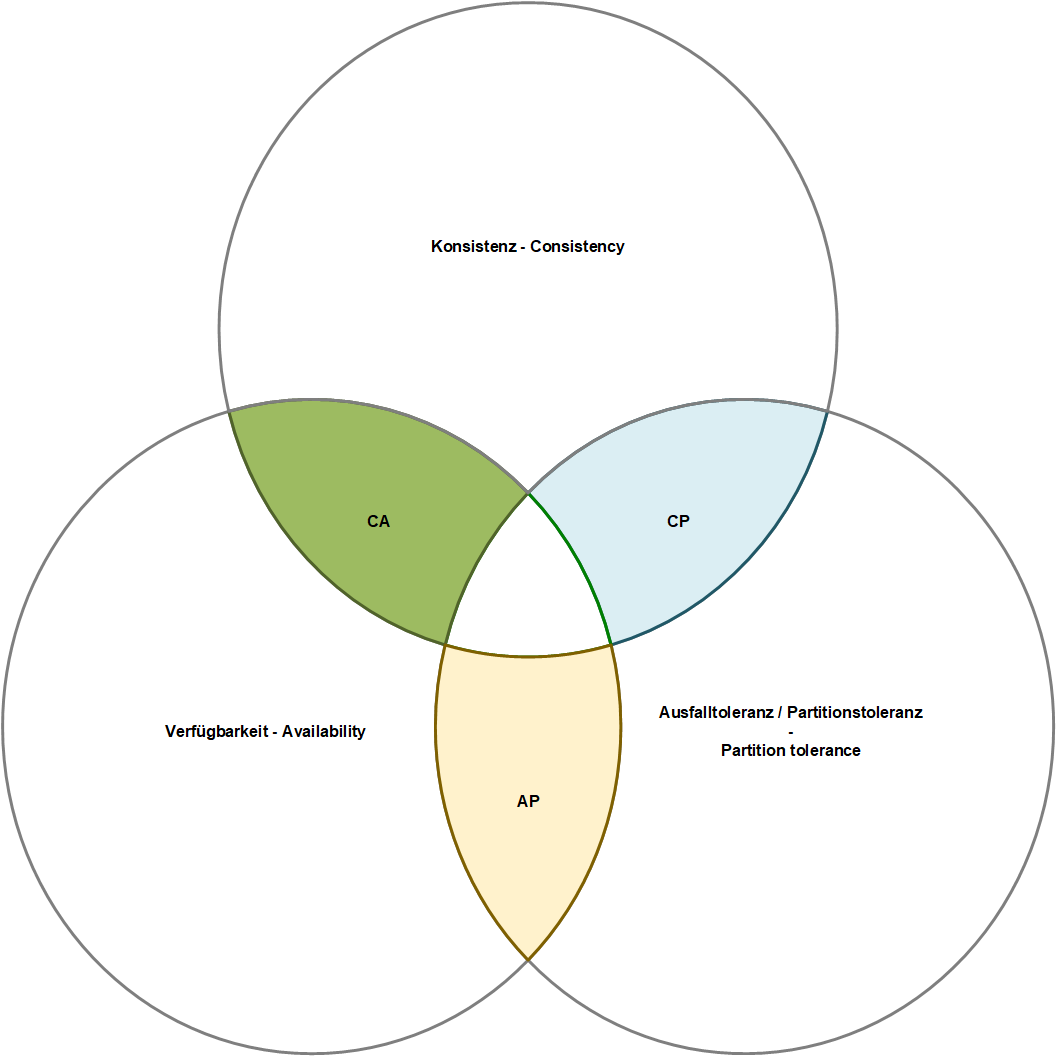
\includegraphics[width=0.5\linewidth]{source/implementation/evaluation/excursus_architecture/cap_theorem}
        \caption{CAP-Theorem}
        \label{fig:cap_theorem}
    \end{figure}

    \Gls{PostgreSQL}, \Gls{Oracle Database} oder \Gls{IBM DB2} präferieren CA, also Konsistenz und Verfügbarkeit.
\end{flushleft}
%! Author = itgramic
%! Date = 05.12.23

% Preamble
\subsubsection{Skalierung}
Datenbanken müssen skalierbar sein.
Dabei wird unterschieden zwischen einer vertikalen Skalierung (scale-up) und horizontaler Skalierung (scale-out).
Bei der vertikalen Skalierung werden den DB-Servern mehr CPU-Cores und Memory sowie zum Teil Storage hinzugefügt, wobei der Storage in jedem Fall wachsen wird.
Beim horizontalen Skalieren werden weitere DB-Nodes in den Cluster eingehängt\cite{IZSGZLVT}:
\begin{figure}[H]
    \centering
    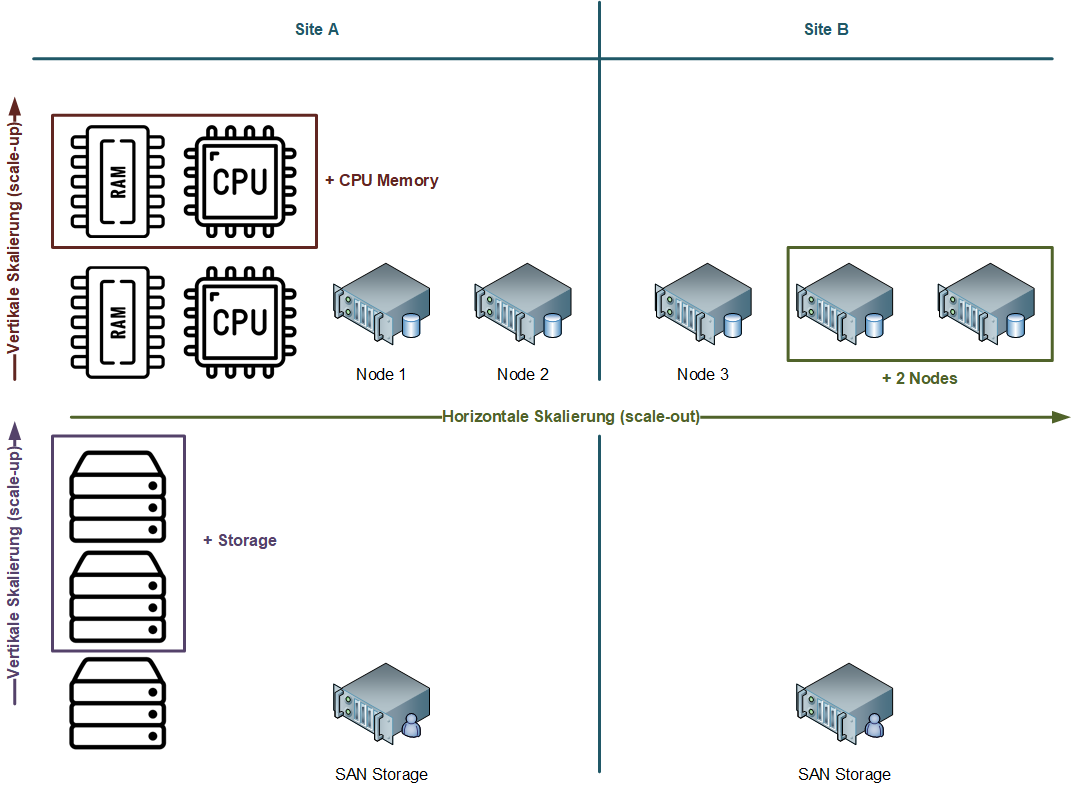
\includegraphics[width=1\linewidth]{source/implementation/evaluation/excursus_architecture/Skalierung}
    \caption{Datenbankskalierung}
    \label{fig:Datenbankskalierung}
\end{figure}

Bei monolithischen Datenbanken, werden irgendwann die grenzen der horizontalen Skalierung erreicht und man muss wieder vertikal Skalieren, um dem Primary Node genügend Rechnerleistung vorzuhalten.
%! Author = itgramic
%! Date = 05.12.23

% Preamble
\subsubsection{Monolithische vs. verteilte SQL Systeme}
Klassische SQL-Datenbanken sind Monolithische Systeme, selbst wenn sie mittels Replikation eine Primary/Standby-Architektur aufweisen.
Man kann mittels eines SQL Proxys ein gewisses Mass an Load Balancing betreiben, hat aber immer noch das Problem das es einen Primary Node gibt auf dem beschrieben wird.

Verteilte Systeme wiederum

\begin{figure}[H]
    \centering
    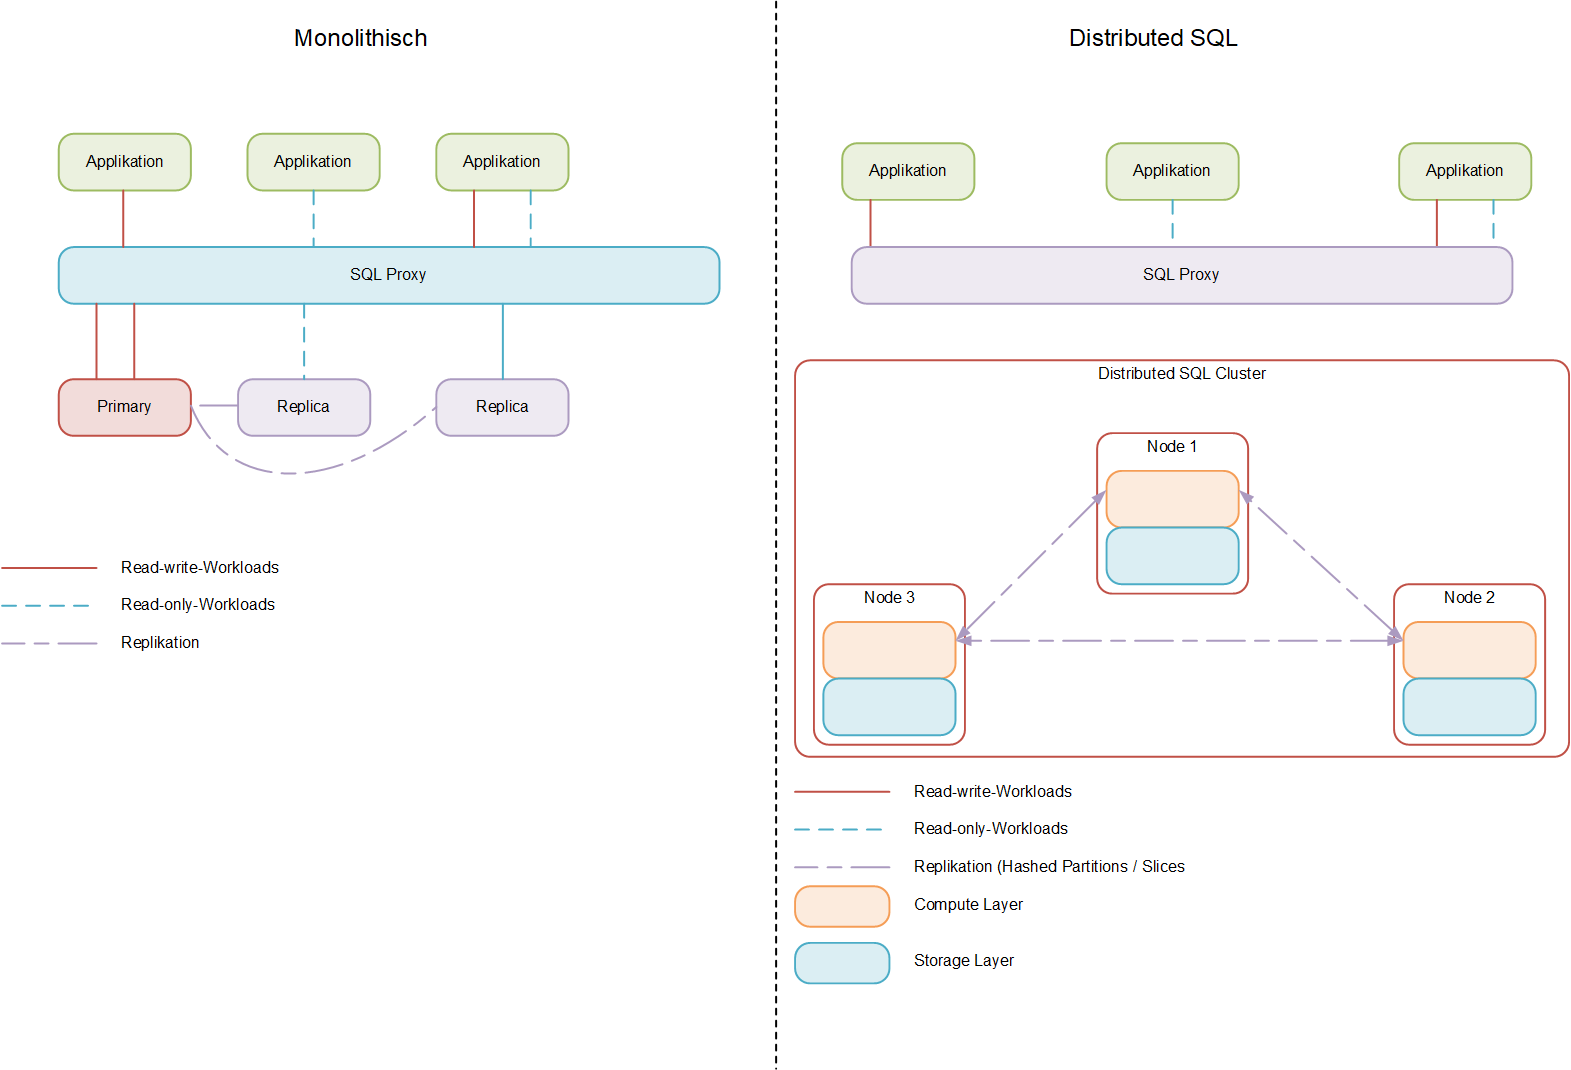
\includegraphics[width=1\linewidth]{source/implementation/evaluation/excursus_architecture/monolith_distributed}
    \caption{Monolithische vs. verteilte SQL Systeme}
    \label{fig:Monolith_vs_Distributed_SQL}
\end{figure}

\subsection{Testziele erarbeiten}
\subsection{PostgreSQL Benchmarking}
PostgreSQL bietet ein Benchmarking-Tool,\cite{TYJFF7AB,VXNYQFTE} mit dem die DB Vermessen werden kann.
\subsection{Analyse gängiger PostgreSQL HA Cluster Lösungen}
%! Author = itgramic
%! Date = 05.12.23

% Preamble
\subsubsection{\Gls{PostgreSQL} Replikation}
PostgreSQL bietet von Haus aus Möglichkeiten, um Replikationen durchzuführen.
Dabei ist nicht jede gleich gut für jedes Szenario geeignet\cite{FZAHA89U}.
%! Author = itgramic
%! Date = 05.12.23

% Preamble
\subsubsection{KSGR Lösung}
Das Kantonsspital Graubünden hat basierend auf \gls{keepalived} wird geprüft ob die primäre Seite erreichbar und betriebsbereit ist.
Trifft dies nicht mehr zu, wird ein \Gls{Failover} durchgeführt\cite{NLF2IDBZ}.
Ist die primäre Seite wieder verfügbar, wird ein Restore auf die primäre Seite gefahren.

Es wird beim Restore immer ein komplettes Backup der sekundären Seite auf die primäre Seite übertragen.
Ursache ist, dass die normalerweise für den Datenrestore benötigten \Gls{PostgreSQL} Board mittel nur für eine relativ kurze Zeit eingesetzt werden können ehe die differenzen zwischen den beiden Seiten zu gross werden.

Bei kleinen Datenbanken wie jene für \Gls{Harbor} und \Gls{GitLab} ist die Zeit die hierfür benötigt wird, nicht relevant.
Sind die Datenbanken auf dem \Gls{PostgreSQL Cluster} jedoch grösser, kann der Restore mehrere Minuten dauern.
%! Author = itgramic
%! Date = 05.12.23

% Preamble
\subsubsection{pgpool-II}
\begin{flushleft}
    pgpool-II ist eine Middleware die zwischen einem \Gls{PostgreSQL Cluster} und einem PostgreSQL-Client gesetzt wird.
\end{flushleft}
\begin{flushleft}
    \paragraph{Core-Features}
    pgpool-II bietet folgende Core-Feature\cite{3XWCD3KX}:
    \begin{itemize}
        \item Watchdog für Automatischer Failover
        \item Eigener \Gls{Quorum}-Algorithmus
        \item Integrierter \Gls{Connection Pooler}
        \item Eigenes Replikationssystem
        \item Integriertes Load Balancing
        \item Limiting Exceeding Connections, also queuen von Connections
        \item In Memory Query Caching
        \item Online Node Recovery / Resynchronisation
    \end{itemize}
\end{flushleft}
\begin{flushleft}
    \paragraph{Replikation}
    pgpool-II bietet ein eigenes Replikationssystem an.
\end{flushleft}
\begin{flushleft}
    Es besteht allerdings die Möglichkeit, die PostgreSQL-Standardreplikationen zu verwenden.
\end{flushleft}
\begin{flushleft}
    \paragraph{Proxy}
    pgpool-II hat bereits einen intergrierten Load Balancer.\\
    Einen zusätzlichen Proxy wird daher nicht benötigt.
\end{flushleft}
\begin{flushleft}
    \paragraph{Pooling}
    pgpool-II bietet ebenfalls von Haus aus einen \Gls{Connection Pooler}.
\end{flushleft}
\begin{flushleft}
    \paragraph{API / Skripte}
    pgpool-II bietet mit \texttt{pgpool} ein eigenes Command- und Toolset an.\\
    Mit dem CLI-Tool \texttt{pcp\_command} bietet pgpool-II zudem über eine abgesicherte API,\\
    die auch via Netzwerk erreichbar ist.
\end{flushleft}
\begin{flushleft}
    \paragraph{Maintenance}
    pgpool-II hat kein GitLab- oder GitHub-Repository.
    Metriken wie die GitHub Insights, welche Aufschluss über den Zustand des Projekts geben, finden sich nicht.
\end{flushleft}
\begin{flushleft}
    Die Dokumentation wird zwar aktualisiert, ist aber sehr minimalistisch gehalten.\\
    Sie bietet nur wenig Informationen zum Aufbau und Architektur von pgpool-II.
\end{flushleft}


%! Author = itgramic
%! Date = 05.12.23

% Preamble
\clearpage
\begin{flushleft}
    \subsubsection{pg\_auto\_failover}
    pg\_auto\_failover ist eine PostgreSQL-Erweiterung, die von der Microsoft Subunternehmen Citus Data entwickelt wird.
\end{flushleft}
\begin{flushleft}
    \paragraph{Core-Features}
    Die wichtigsten Features von pg\_auto\_failover sind:
    \begin{itemize}
        \item API
        \item PostgreSQL Extension, also reines PostgreSQL
        \item State Machine Driven
        \item Replikations-Quorum
        \item Citus kompatibel
        \item Azure VM Support
    \end{itemize}
\end{flushleft}
\begin{flushleft}
    \paragraph{Replikation}
    pg\_auto\_failover bietet die Standard PostgreSQL-Replikationen.
\end{flushleft}
\begin{flushleft}
    \paragraph{Proxy}
    pg\_auto\_failover benötigt einen \Gls{HAProxy}, um Load Balancing betreiben zu können  \cite{VYXTI7BS}.
\end{flushleft}
\begin{flushleft}
    \paragraph{API / Skripte}
    pg\_auto\_failover bietet ein eigenes CLI-Tool, \texttt{pg\_autoctl}.
    Dieses stellt Commands für das Einbinden neuer Nodes,
    das Managen von Nodes (Maintenance resp. Switchover),\\
    Konfigurieren oder Monitoren des Systems zur Verfügung \cite{4X2AKDB6}.
\end{flushleft}
\clearpage
\begin{flushleft}
    \paragraph{Architektur}
    Die Dokumentation resp. Grafik von pg\_auto\_failover  \cite{PZZIZ5RT} zeigt auf, wie der Failover funktioniert:
    \begin{figure}[H]
        \centering
        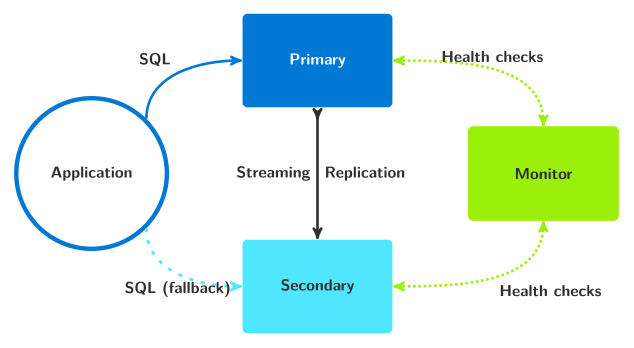
\includegraphics[width=0.75\linewidth]{source/implementation/evaluation/postgresql_ha_solutions/pg_auto_failover/pg_auto-failover_arch-single-standby}
        \caption{pg\_auto\_failover-Architektur - Single Standby}
        \label{fig:pg_auto-failover_arch-single-standby}
    \end{figure}
    Aber wie die Grafik zeigt, können auch Multi-Nodes können eingebunden werden \cite{4ZKBDG57}:
    \begin{figure}[H]
        \centering
        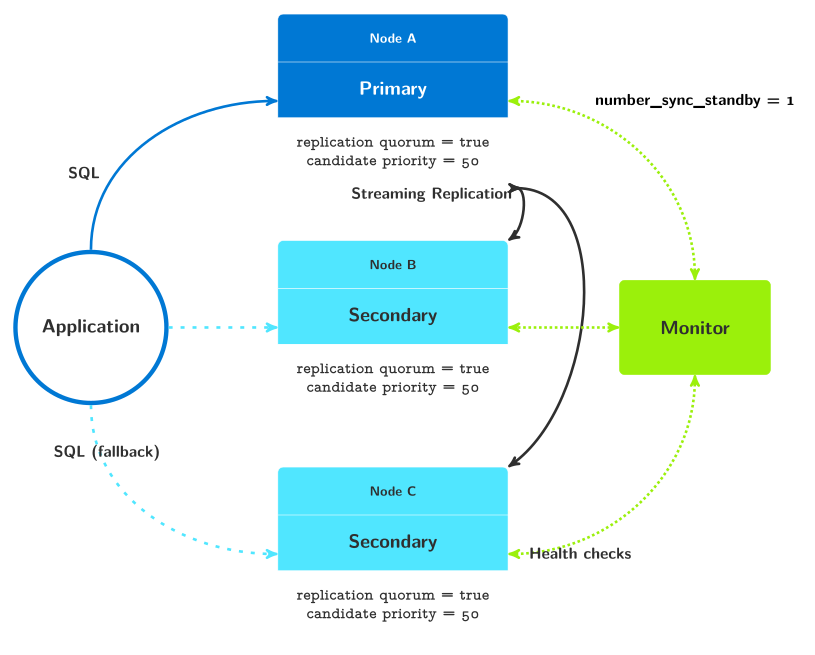
\includegraphics[width=0.75\linewidth]{source/implementation/evaluation/postgresql_ha_solutions/pg_auto_failover/pg_auto-failover_arch-multi-standby}
        \caption{pg\_auto\_failover-Architektur - Multi-Node Standby}
        \label{fig:pg_auto-failover_arch-multi-standby}
    \end{figure}
    \clearpage
    pg\_auto\_failover kann Citus einbinden.
    Allerdings bleibt die Architektur im Kern immer monolithisch.\\
    Die nachfolgende Grafik zeigt die Architektur mit Citus \cite{3FVHLIFE}:
    \begin{figure}[H]
        \centering
        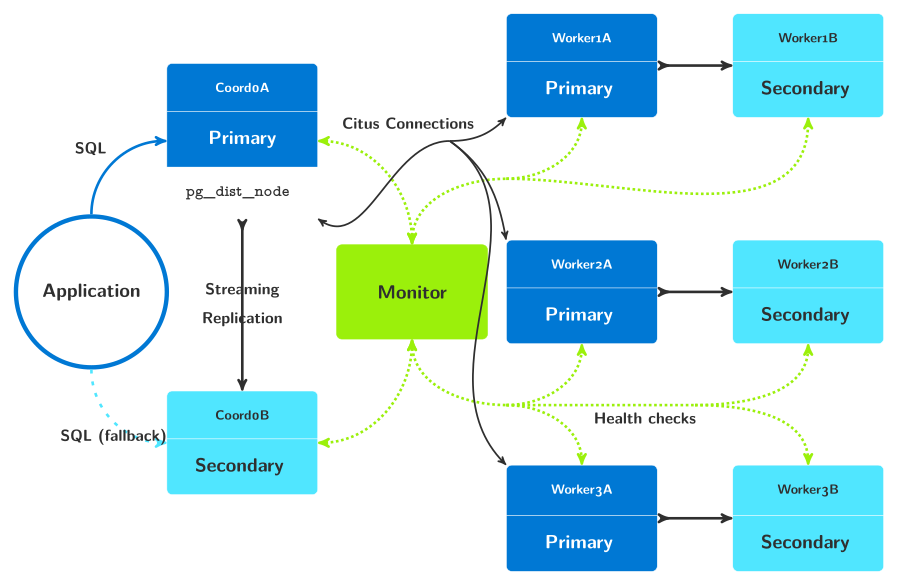
\includegraphics[width=0.75\linewidth]{source/implementation/evaluation/postgresql_ha_solutions/pg_auto_failover/pg_auto-failover_arch-citus}
        \caption{pg\_auto\_failover-Architektur - Citus}
        \label{fig:pg_auto-failover_arch-citus}
    \end{figure}
\end{flushleft}
\begin{flushleft}
    \paragraph{Synergien und Mehrwert}
    pg\_auto\_failover bietet eine Docker-Compose-Integration.\\
    Allerdings ist keine Kubernetes-Integration dokumentiert.
\end{flushleft}
\begin{flushleft}
    Damit bietet pg\_auto\_failover keine Möglichkeit\\
    Synergien zwischen monolithischer Architektur und einer Cloud-Native-Umsetzung auf Kubernetes.\\
    Entsprechend ist kein Mehrwert vorhanden.
\end{flushleft}
%! Author = itgramic
%! Date = 05.12.23

% Preamble
\clearpage
\begin{flushleft}
    \subsubsection{Patroni}
    Patroni ist eine von Zalando auf Basis von Python entwickelte HA-Lösung für \Gls{PostgreSQL}.\\
    Patroni wird aktiv von Zalando gepflegt.
\end{flushleft}
\begin{flushleft}
    \paragraph{Core-Features}
    Patroni bietet folgende Core-Features:
    \begin{itemize}
        \item Rest-API und eigenes Skript- und Toolset
        \item Aktionen und Konfigurationen im Konsensprinzip abgestimmt
        \item Manueller oder Sheduled Switchover
        \item Reines PostgreSQL als Basis, Patroni setzt Hilfe von Python darauf auf
        \item Automatische reintegration von Nodes nach einem Fehler
        \item Citus kompatibel
        \item Docker und Docker-compose Dokumentation
    \end{itemize}
\end{flushleft}
\begin{flushleft}
    \paragraph{Replikation}
    Patroni bietet per Default eine eigene Replikation an.\\
    Diese ist allerdings eine asynchrone Replikation.
\begin{flushleft}
    Patroni unterstützt aber die synchrone Replikation von \Gls{PostgreSQL}.
\end{flushleft}
\end{flushleft}
\begin{flushleft}
    \paragraph{Proxy}
    Patroni benötigt einen \Gls{HAProxy}, um Load Balancing betreiben zu können\cite{VYXTI7BS}.
\end{flushleft}
\begin{flushleft}
    \paragraph{Pooling}
    Patroni benötigt einen externen \Gls{Connection Pooler}.\\
    Hier wird oft PgBouncer \cite{ATBELZ2X} verwendet.
\end{flushleft}
\begin{flushleft}
    \paragraph{API / Skripte}
    Patroni hat ein eigenes Tool- und Commandset, \texttt{patronictl}, welches die Verwaltung vereinfacht.\\
    Es umfasst das Ändern und Erfassen von Konfigurationen, das Forcieren eines Failovers als Switchover, Maintenance Handling und Informationsbeschaffung.\\
    Zusätzlich bietet Patroni eine API, welche Daten für das Monitoring bereitstellt,\\
    aber auch Betriebsfunktionen zur Verfügung stellt.\\
\end{flushleft}
\begin{flushleft}
    \paragraph{\gls{etcd}}
    Patroni benötigt etcd oder \Gls{Consul} als \Gls{Key-Value-Store}.
\end{flushleft}
\begin{flushleft}
    \paragraph{Architektur}
    Das Architektur-Schaubild sieht folgendermassen aus:
    \begin{figure}[H]
        \centering
        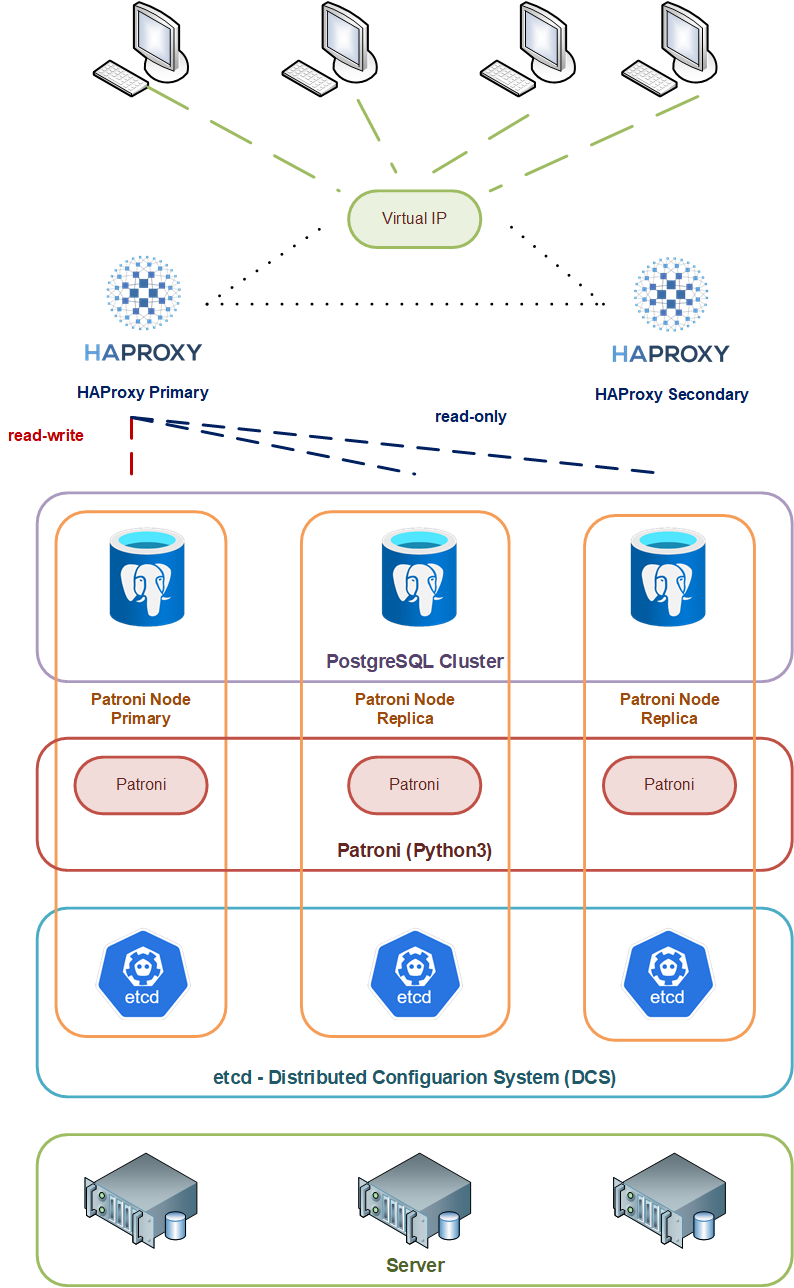
\includegraphics[width=0.7\linewidth]{source/implementation/evaluation/postgresql_ha_solutions/patroni_architecture}
        \caption{Patroni-Architektur}
        \label{fig:patroni-architecture}
    \end{figure}
\end{flushleft}
\begin{flushleft}
    \paragraph{Maintenance}
    Patroni ist ein sehr gepflegtes Projekt, welches die gängigen Community Standards einhält.\\
    Die Details sind im \hyperref[subsec:maintenance_patroni]{Anhang - Maintenance} zu finden.
\end{flushleft}
\begin{flushleft}
    \paragraph{Synergien und Mehrwert}
    Patroni kann nicht nur mit Citus zu einem Distributed / Sharded SQL System umgebaut werden,\\
    es ist auch Kern von StackGres.
\end{flushleft}
\begin{flushleft}
    Damit könnten die API und Skripte in beiden Welten verwendet werden.\\
    Der Aufwand für die Verwaltung und Optimierung würde stark gesenkt.\\
    Projekte wie \texttt{vitabaks / postgresql\_cluster}\cite{HIQVBEPF} bieten zudem die Vorlage für eine noch stärkere Automatisierung.
\end{flushleft}
%! Author = itgramic
%! Date = 05.12.23

% Preamble
\begin{flushleft}
    \subsubsection{CloudNativePG}
    CloudNativePG ist eine Containerlösung für PostgreSQL auf Kubernetes.
\end{flushleft}
\begin{flushleft}
    \paragraph{Core-Features}
    Die wichtigsten Features von CloudNativePG sind\cite{5ALQPE2U}:
    \begin{description}
        \item k8s API integration
        \item Autoamtischer Failover
        \item Self-Healing von Nodes resp. Replikas
        \item Skalierbarkeit (Vertikal, Horizontal bedingt)
        \item Volumne Backup
        \item Object Backup
        \item Rolling PostgreSQL Upgrade / Updates
        \item Pooling mit PgBouncer
        \item Offline und Online Import von bestehenden PostgreSQL DBs
    \end{description}
\end{flushleft}
\begin{flushleft}
    \paragraph{Replikation}
    CloudNativePG bietet die üblichen PostgreSQL Replikaionen an.
\end{flushleft}
\begin{flushleft}
    \paragraph{Proxy}
    CloudNativePG benötigt keinen zusätzlichen Proxy.
\end{flushleft}
\begin{flushleft}
    \paragraph{Pooling}
    CloudNativePG unterstützt pgBouncer als Pooler.
\end{flushleft}
\begin{flushleft}
    \paragraph{API / Skripte}
    CloudNativePG bietet eine API zum Monitoren und Verwalten von Backups, Clustern und dem System selbst\cite{L7PXKAUY}.
\end{flushleft}
\begin{flushleft}
    \paragraph{Architektur}
    Kubernetes regelt die Zugriffe mittels eines entsprechenden Services in die Nodes auf den Pods:
    \begin{figure}[H]
        \centering
        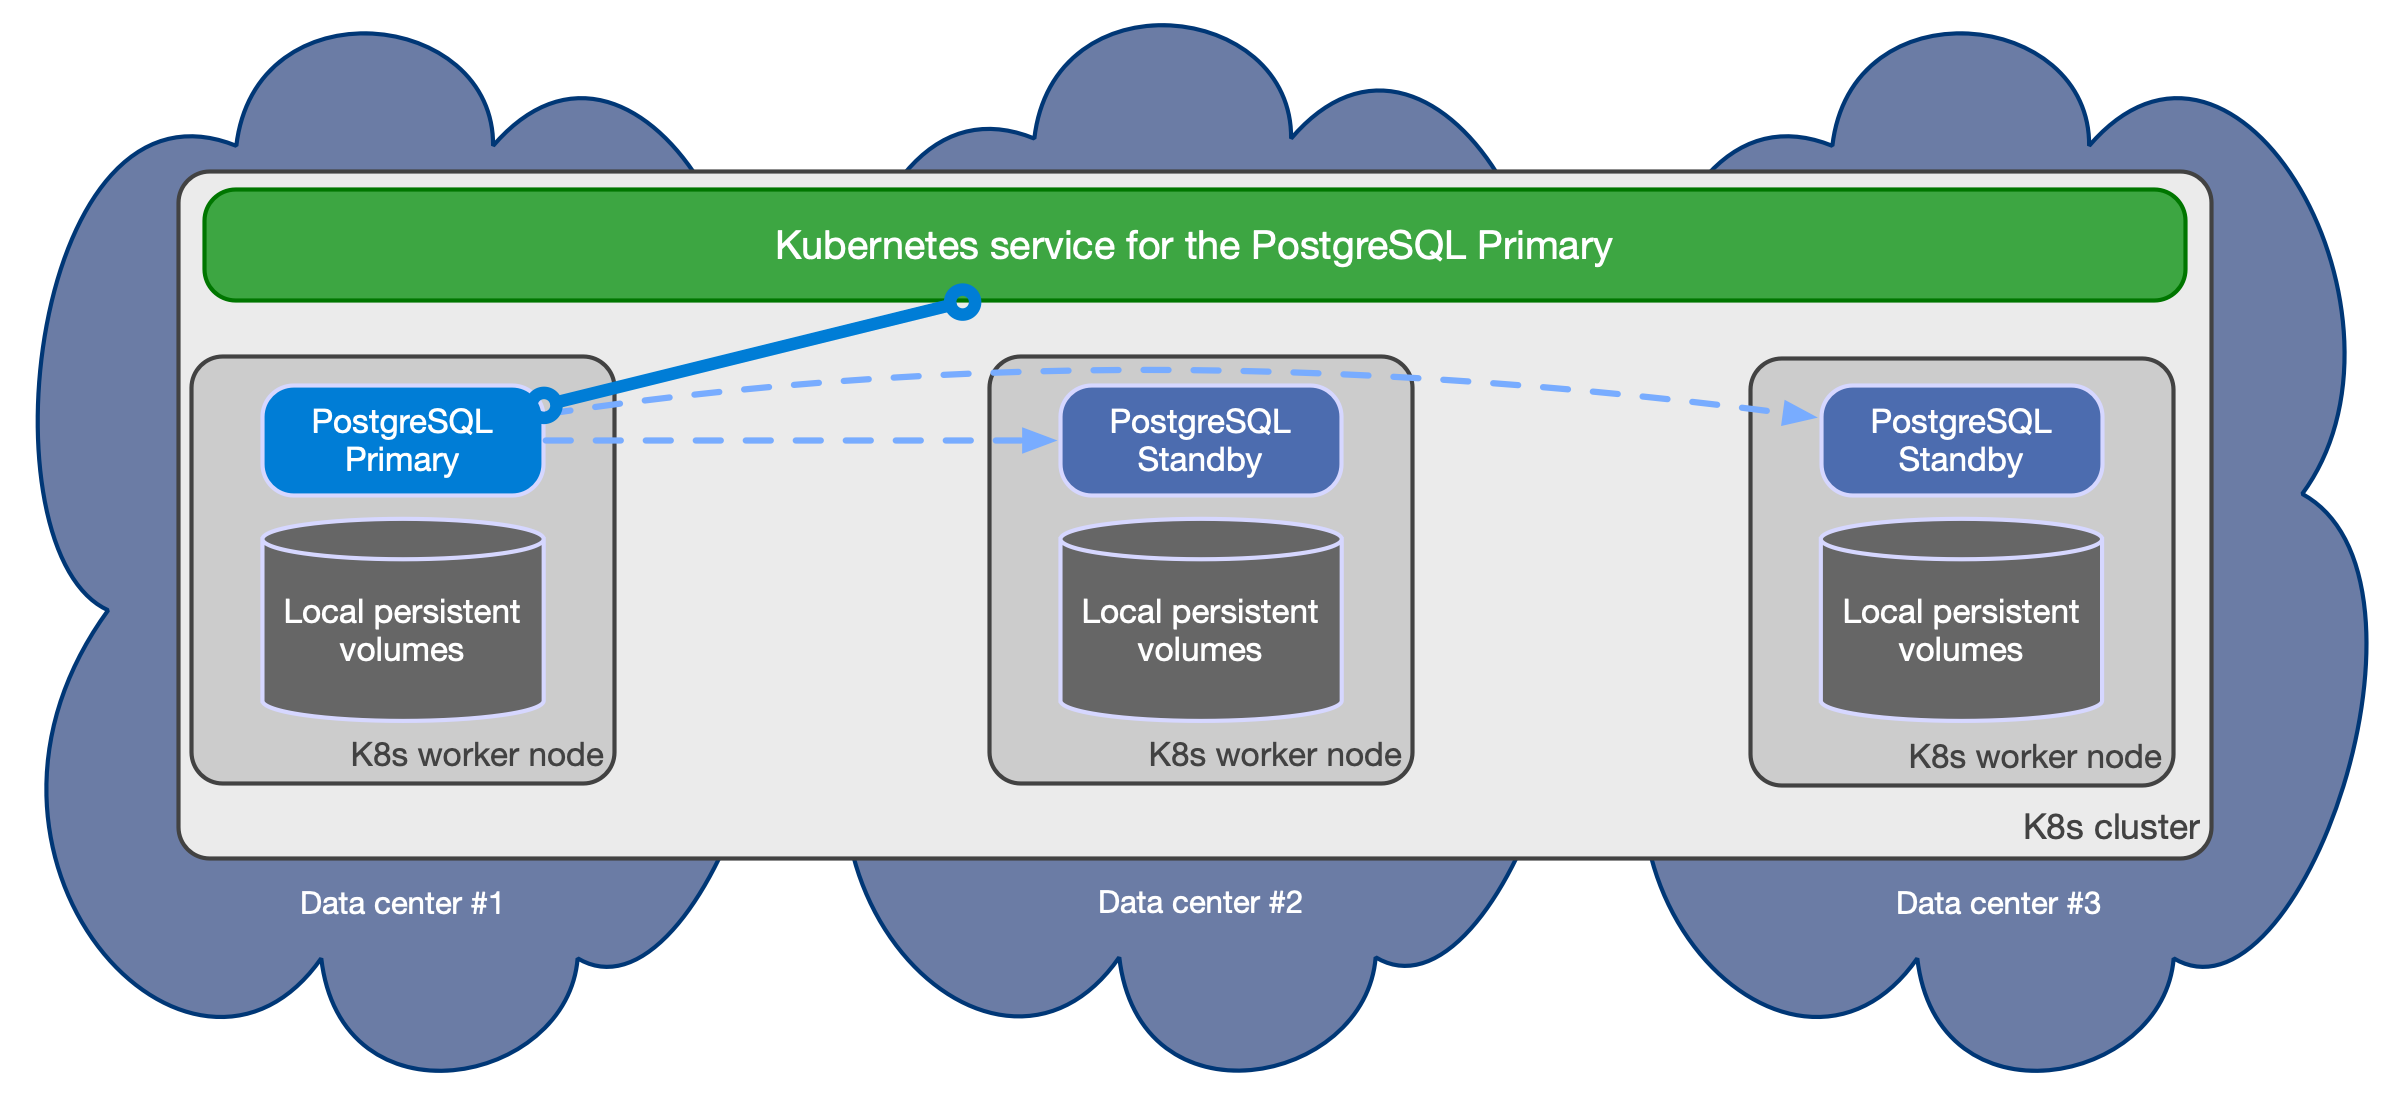
\includegraphics[width=0.75\linewidth]{source/implementation/evaluation/postgresql_ha_solutions/cloudnativepg/k8s-pg-architecture}
        \caption{CloudNativePG - Kubernetes - PostgreSQL}
        \label{fig:k8s-pg-architecture}
    \end{figure}
\end{flushleft}
\begin{flushleft}
    Dabei werden die Read-write workloads an den Primary Node gesendet:
    \begin{figure}[H]
        \centering
        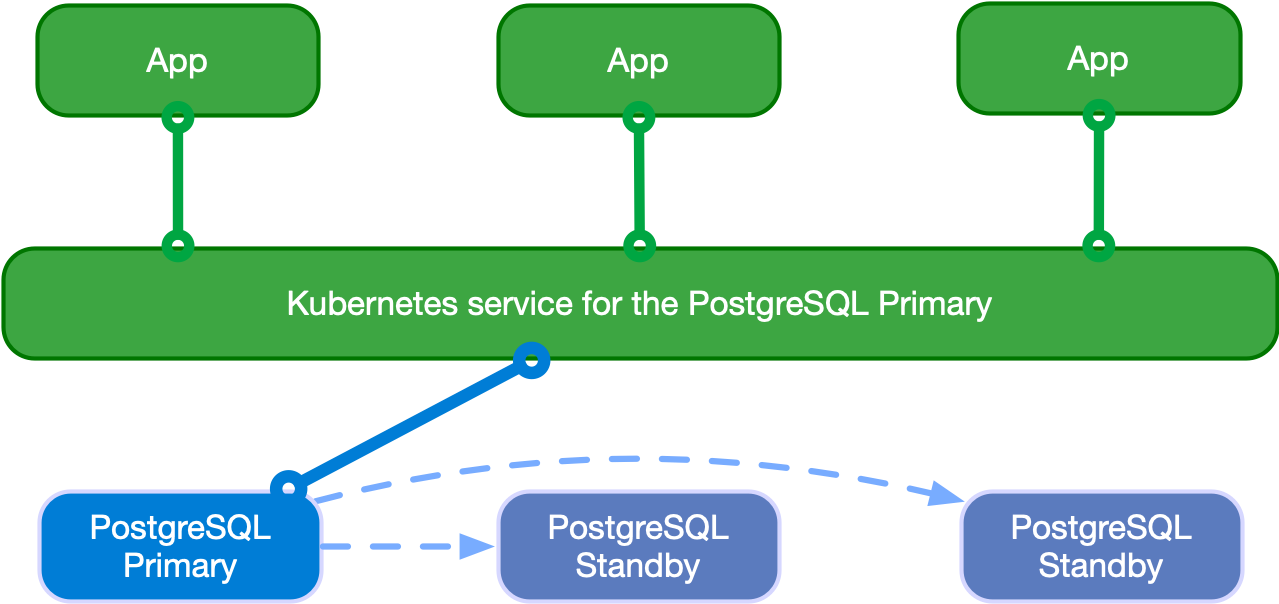
\includegraphics[width=0.75\linewidth]{source/implementation/evaluation/postgresql_ha_solutions/cloudnativepg/cloudnativepg-architecture-rw}
        \caption{CloudNativePG - Kubernetes - Read-write workloads}
        \label{fig:cloudnativepg-architecture-rw}
    \end{figure}
\end{flushleft}
\begin{flushleft}
    Read-only workloads werden mit Round robin an die Replikas zugewiesen:
    \begin{figure}[H]
        \centering
        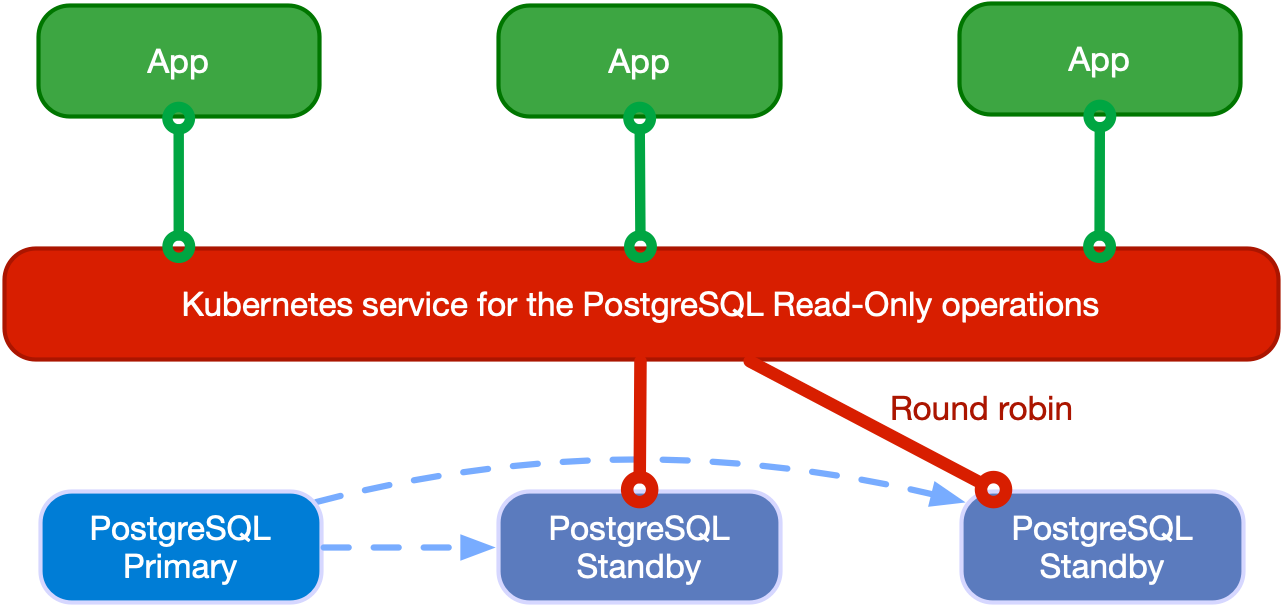
\includegraphics[width=0.75\linewidth]{source/implementation/evaluation/postgresql_ha_solutions/cloudnativepg/cloudnativepg-architecture-read-only}
        \caption{CloudNativePG - Kubernetes - Read-only workloads}
        \label{fig:cloudnativepg-architecture-read-only}
    \end{figure}
\end{flushleft}
\begin{flushleft}
    Es könnten auch Lösungen mit Designated Kubernetes-Clustern in einem anderen RZ oder einer anderen Geo-Region relaisiert werden.
\end{flushleft}
\begin{flushleft}
    \paragraph{Maintenance}
\end{flushleft}
\begin{flushleft}
    \paragraph{Synergien und Mehrwert}
    CloudNativePG bleibt ein Monolithisches System,\\welches aber keine Möglichkeit bietet,\\auch auf einem Normalen Serversetting betrieben zu werden.
\end{flushleft}
\begin{flushleft}
    Daher bietet CloudNativePG weder einen Benefit durch seine Architektur noch mit der Möglichkeit,\\Synergien nutzen zu können.
\end{flushleft}
%! Author = gramic
%! Date = 22.04.24

% Preamble
\begin{flushleft}
    \subsection{YugabyteDB}
    \label{subsec:appendix_testing_yugabytedb}
    Zum einen kann der Fehler irgendwann auftreten.\\
    In diesem Fall wird erst im Log die Fehlermeldung geworfen, dass die Zeitdifferenz zu gross ist:
    \begin{figure}[H]
        \centering
        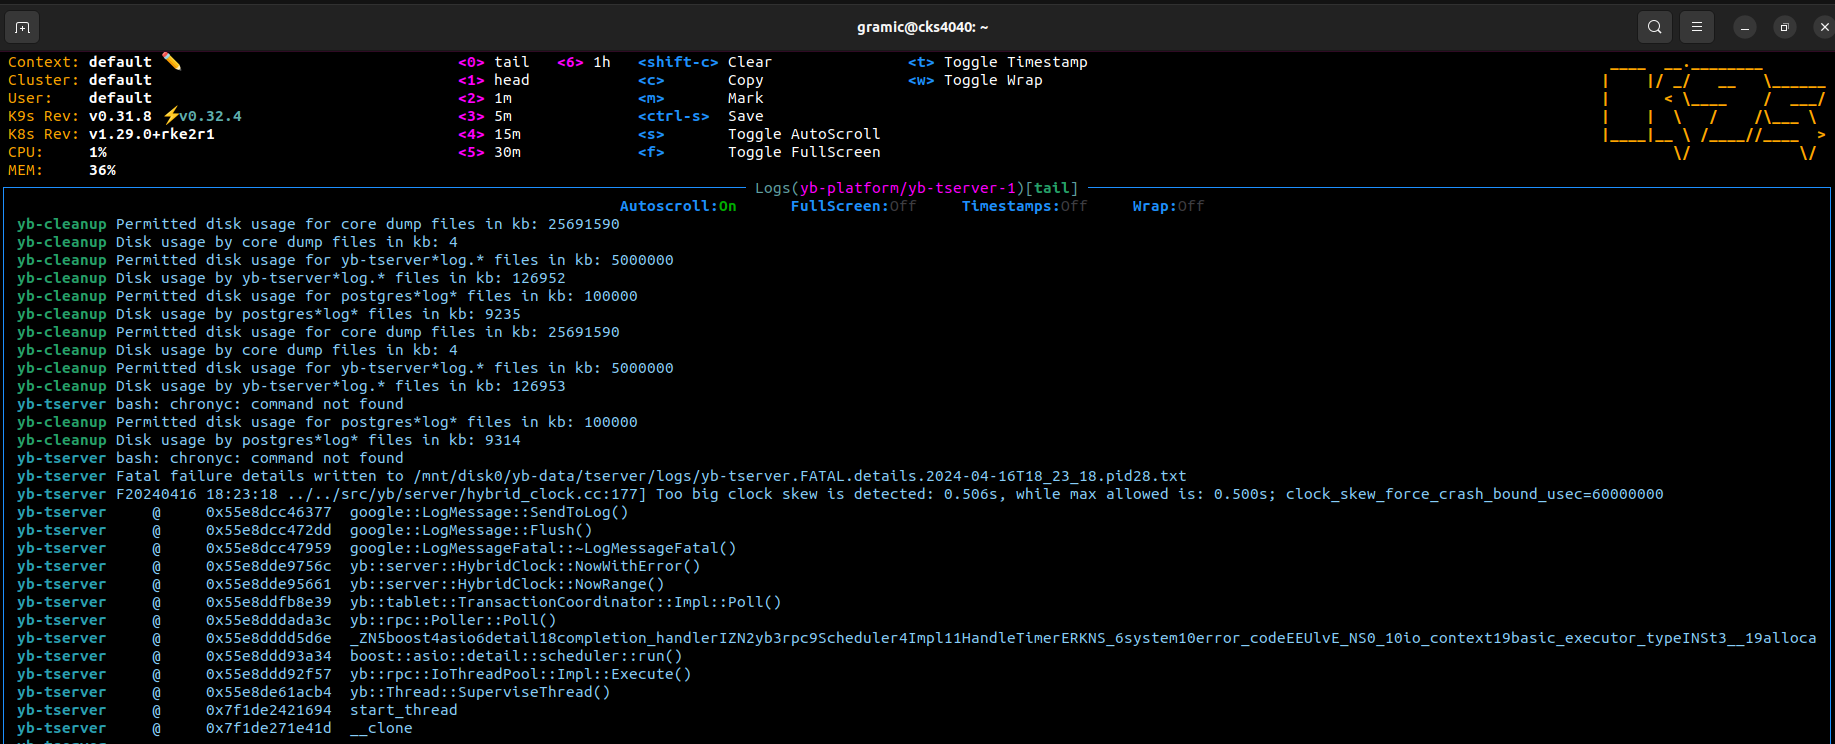
\includegraphics[width=1\linewidth]{source/appendix/evaluation_testing/yugabytedb_too_big_clock_skew_is_detected}
        \caption{YugabyteDB - Too big clock skew is detected}
        \label{fig:yugabytedb_too_big_clock_skew_is_detected}
    \end{figure}
    Eine Folge ist, dass kein neuer Leader bestimmt werden kann:
    \begin{figure}[H]
        \centering
        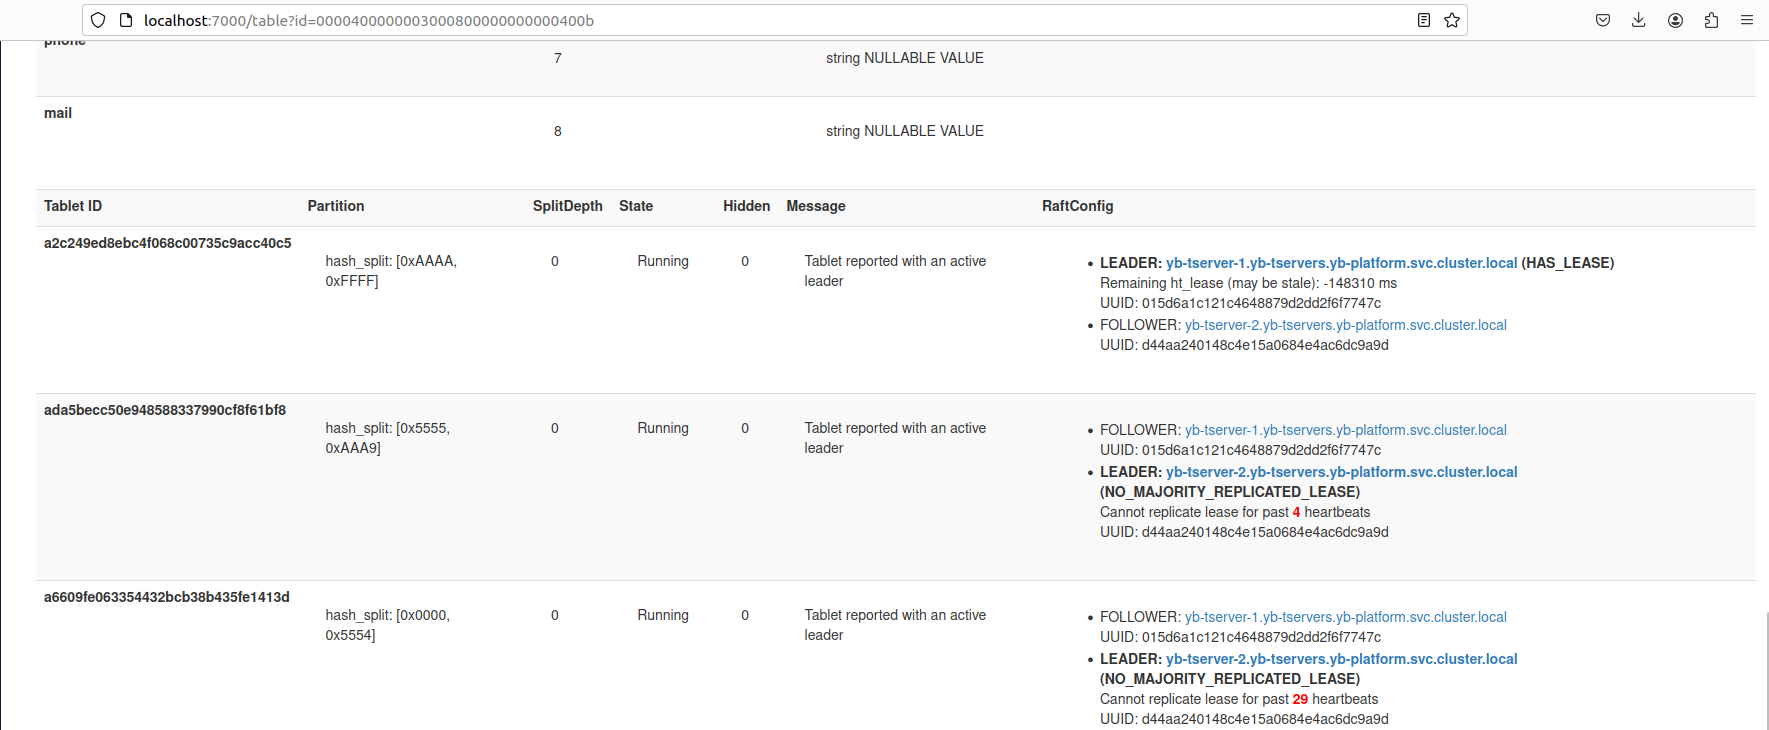
\includegraphics[width=1\linewidth]{source/appendix/evaluation_testing/yugabytedb_tablet_leader_lease}
        \caption{YugabyteDB - Tablet Leader - No Lease}
        \label{fig:yugabytedb_tablet_leader_lease}
    \end{figure}
    Als nächstes wird der komplette \texttt{tserver} in einem \texttt{CrashLoopBackOff} fallen:
    \begin{figure}[H]
        \centering
        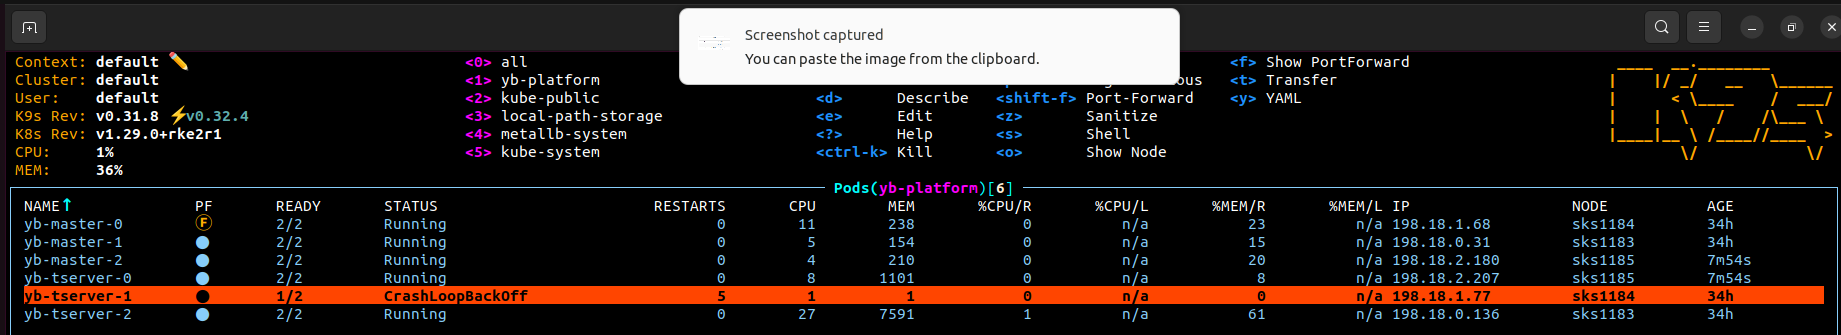
\includegraphics[width=1\linewidth]{source/appendix/evaluation_testing/yugabytedb_crashloopbackoff}
        \caption{YugabyteDB - CrashLoopBackOff}
        \label{fig:yugabytedb_crashloopbackoff}
    \end{figure}
    Der ganze Cluster an sich aber bleibt arbeitsfähig.
\end{flushleft}
\begin{flushleft}
    Anders sieht es aus, wenn auch \texttt{tmaster}-Nodes von Start weg betroffen sind.\\
    Es werden aber primär nur die Logs überall geschrieben:
    \begin{figure}[H]
        \centering
        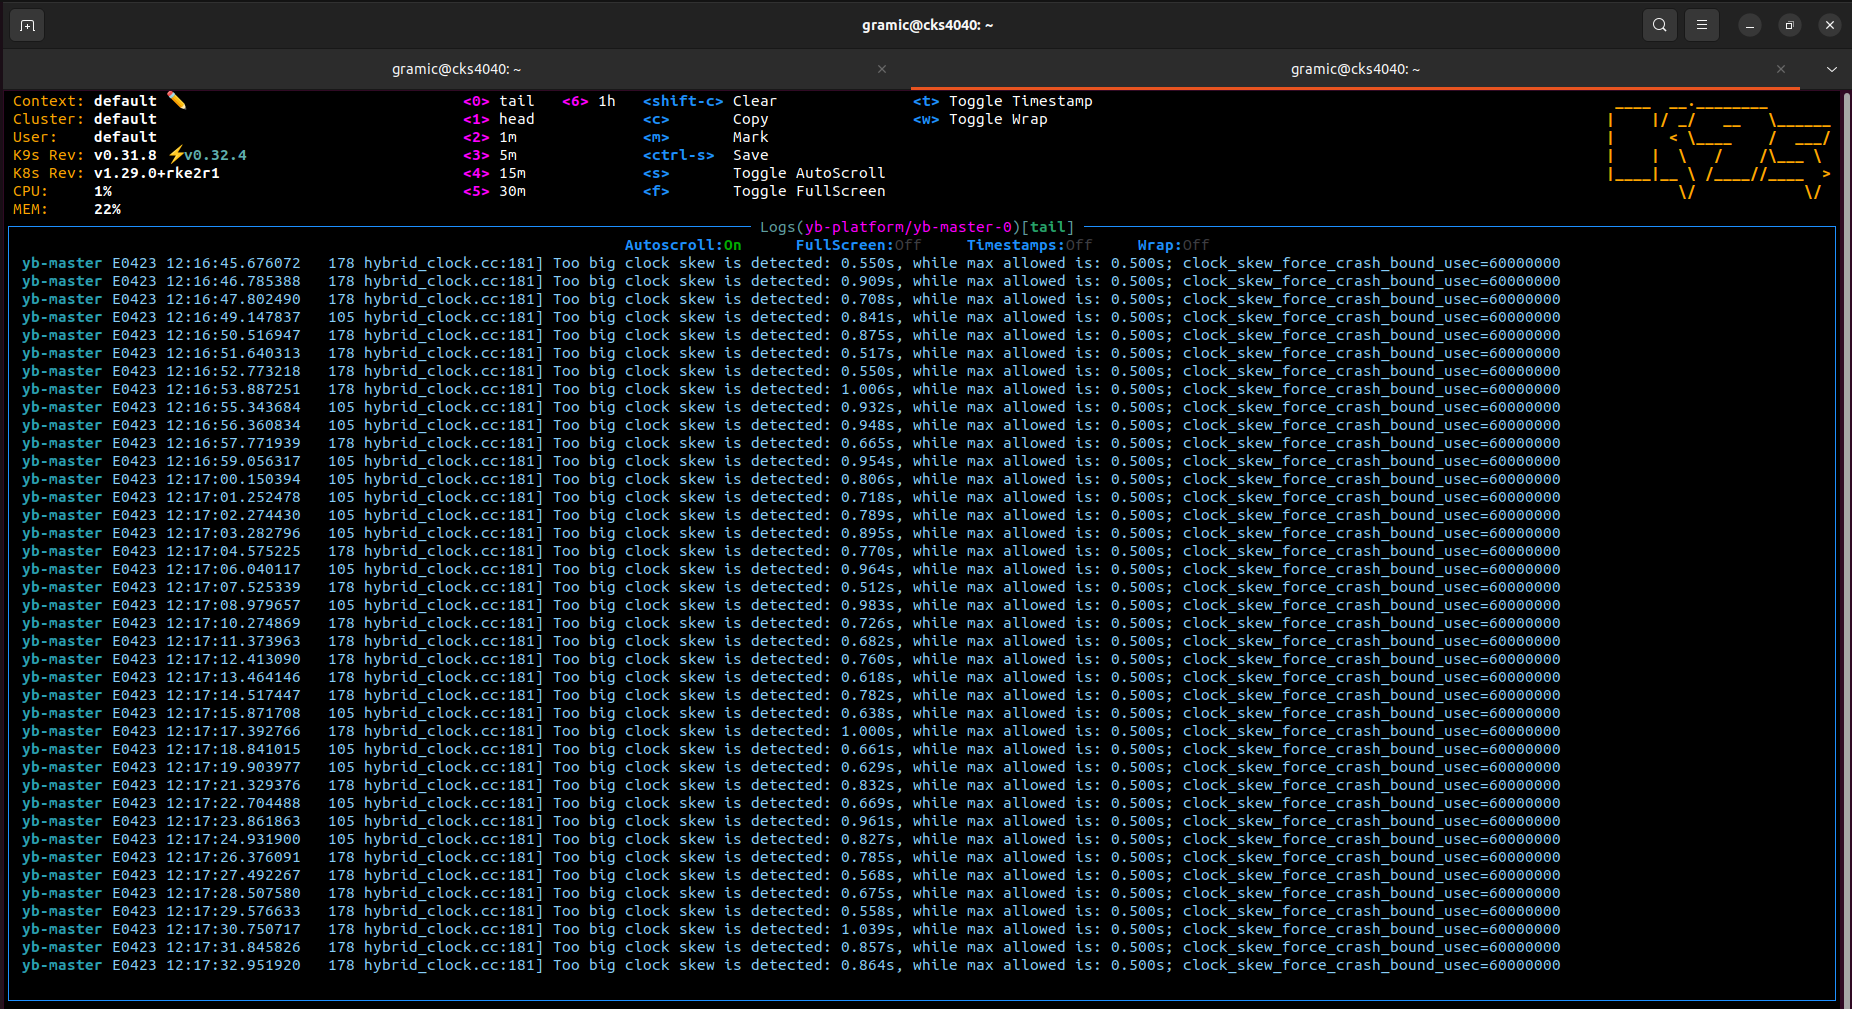
\includegraphics[width=1\linewidth]{source/appendix/evaluation_testing/yugabytedb_yb-tmaster-0_sks1184_clock_error}
        \caption{YugabyteDB - Too big clock skew is detected - tmaster}
        \label{fig:yugabytedb_yb-tmaster-0_sks1184_clock_error}
    \end{figure}
    \begin{figure}[H]
        \centering
        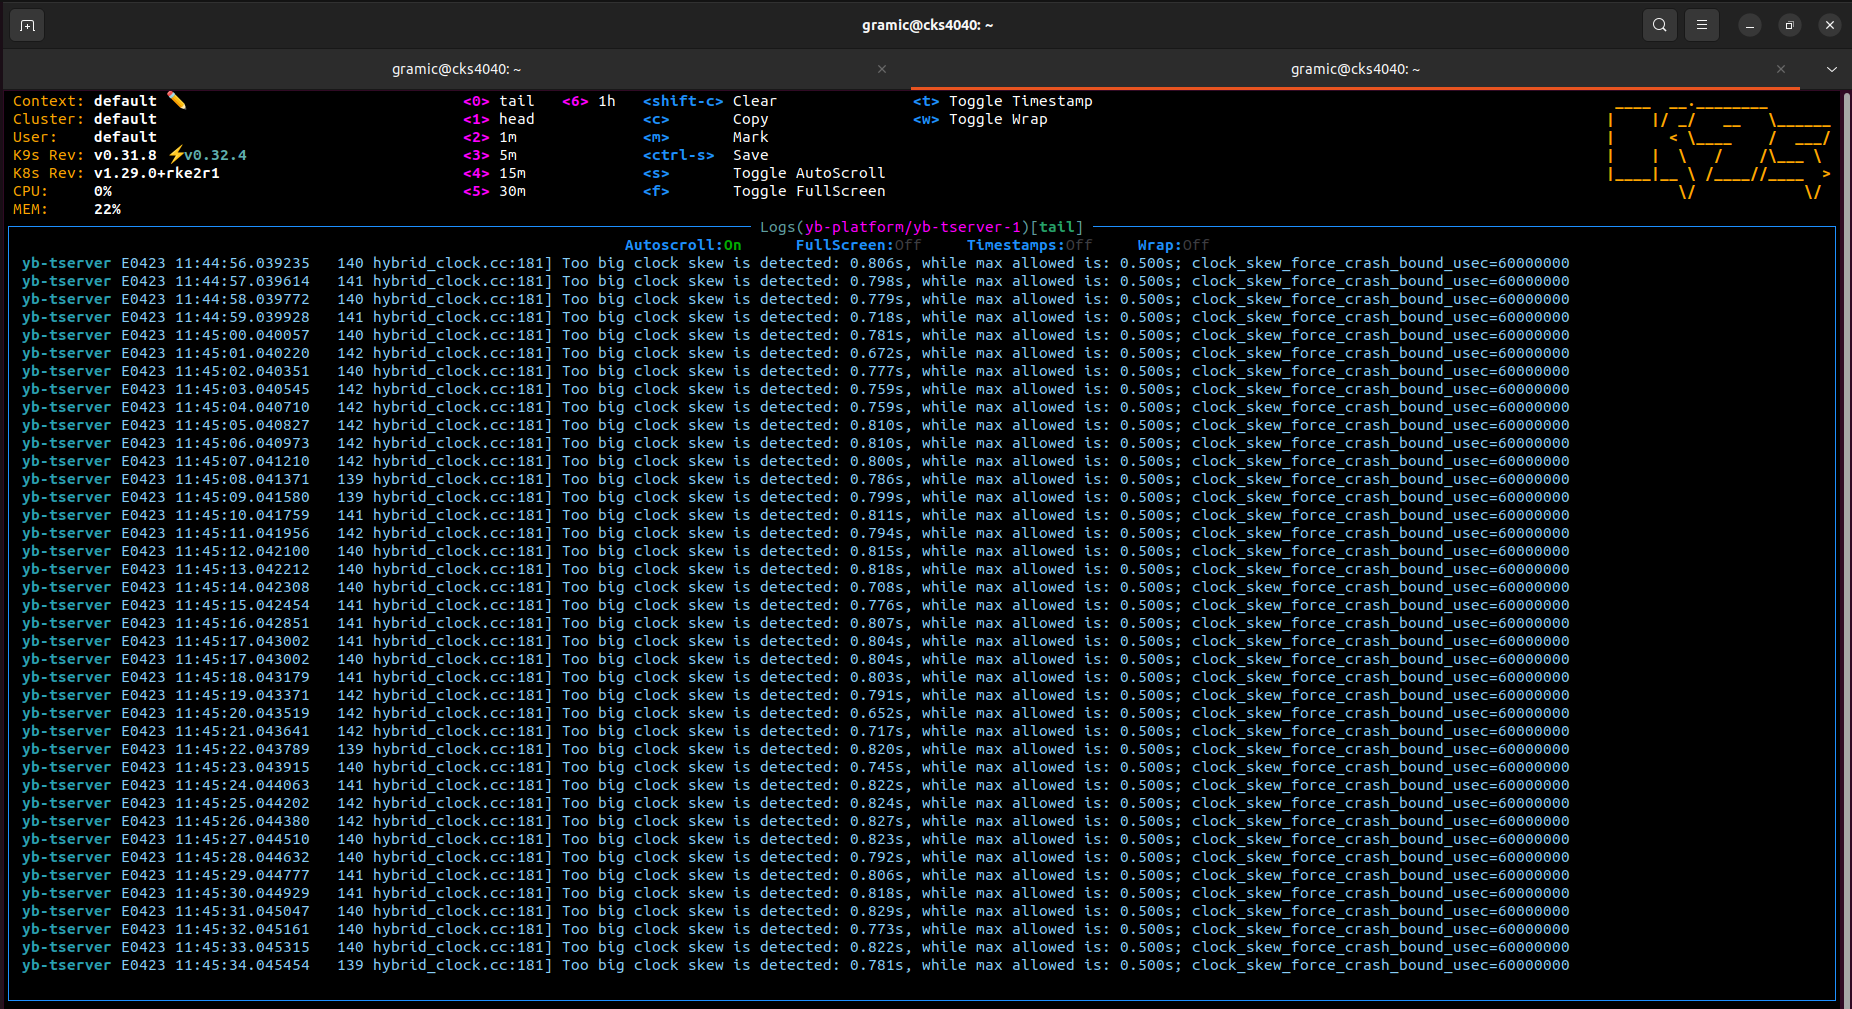
\includegraphics[width=1\linewidth]{source/appendix/evaluation_testing/yugabytedb_yb-tserver-1_sks1184_clock_error}
        \caption{YugabyteDB - Too big clock skew is detected - tserver}
        \label{fig:yugabytedb_yb-tserver-1_sks1184_clock_error}
    \end{figure}
%    \begin{figure}[H]
%        \centering
%        \subfloat[yb-tmaster-0]{{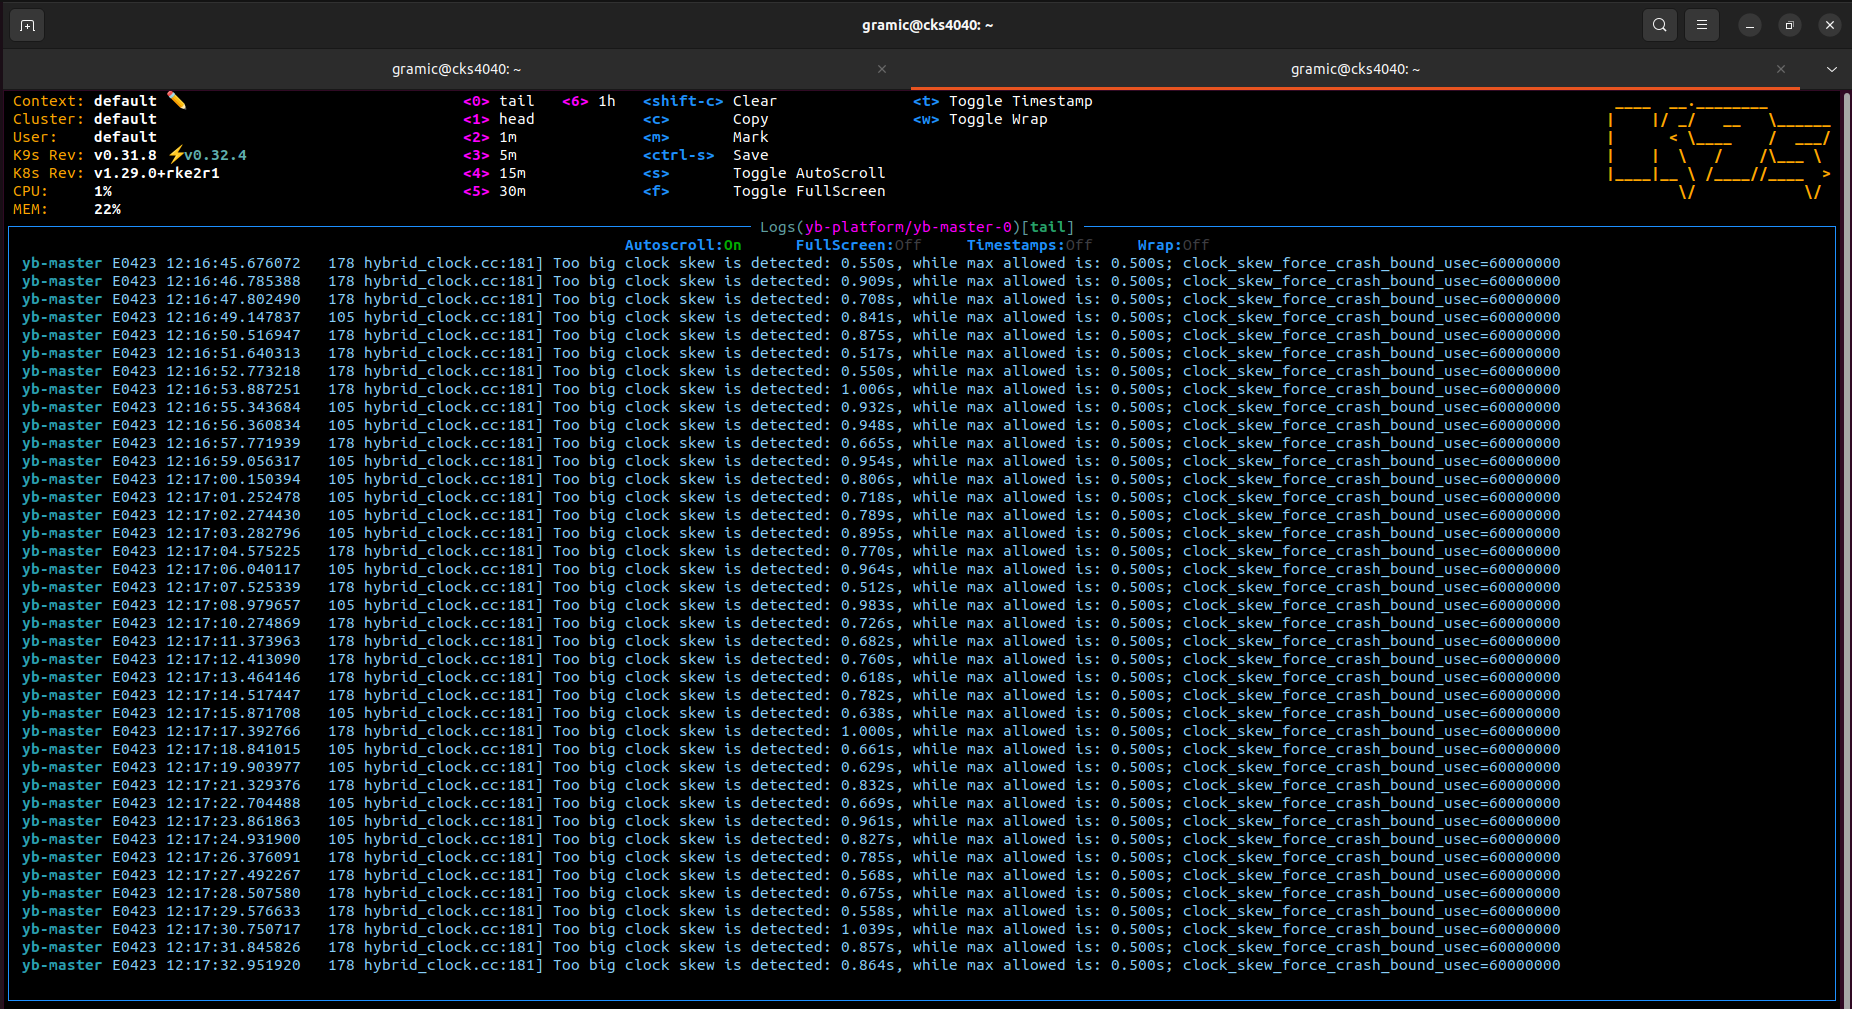
\includegraphics[width=0.47\linewidth]{source/appendix/evaluation_testing/yugabytedb_yb-tmaster-0_sks1184_clock_error} }}%
%        \qquad
%        \subfloat[yb-tserver-1]{{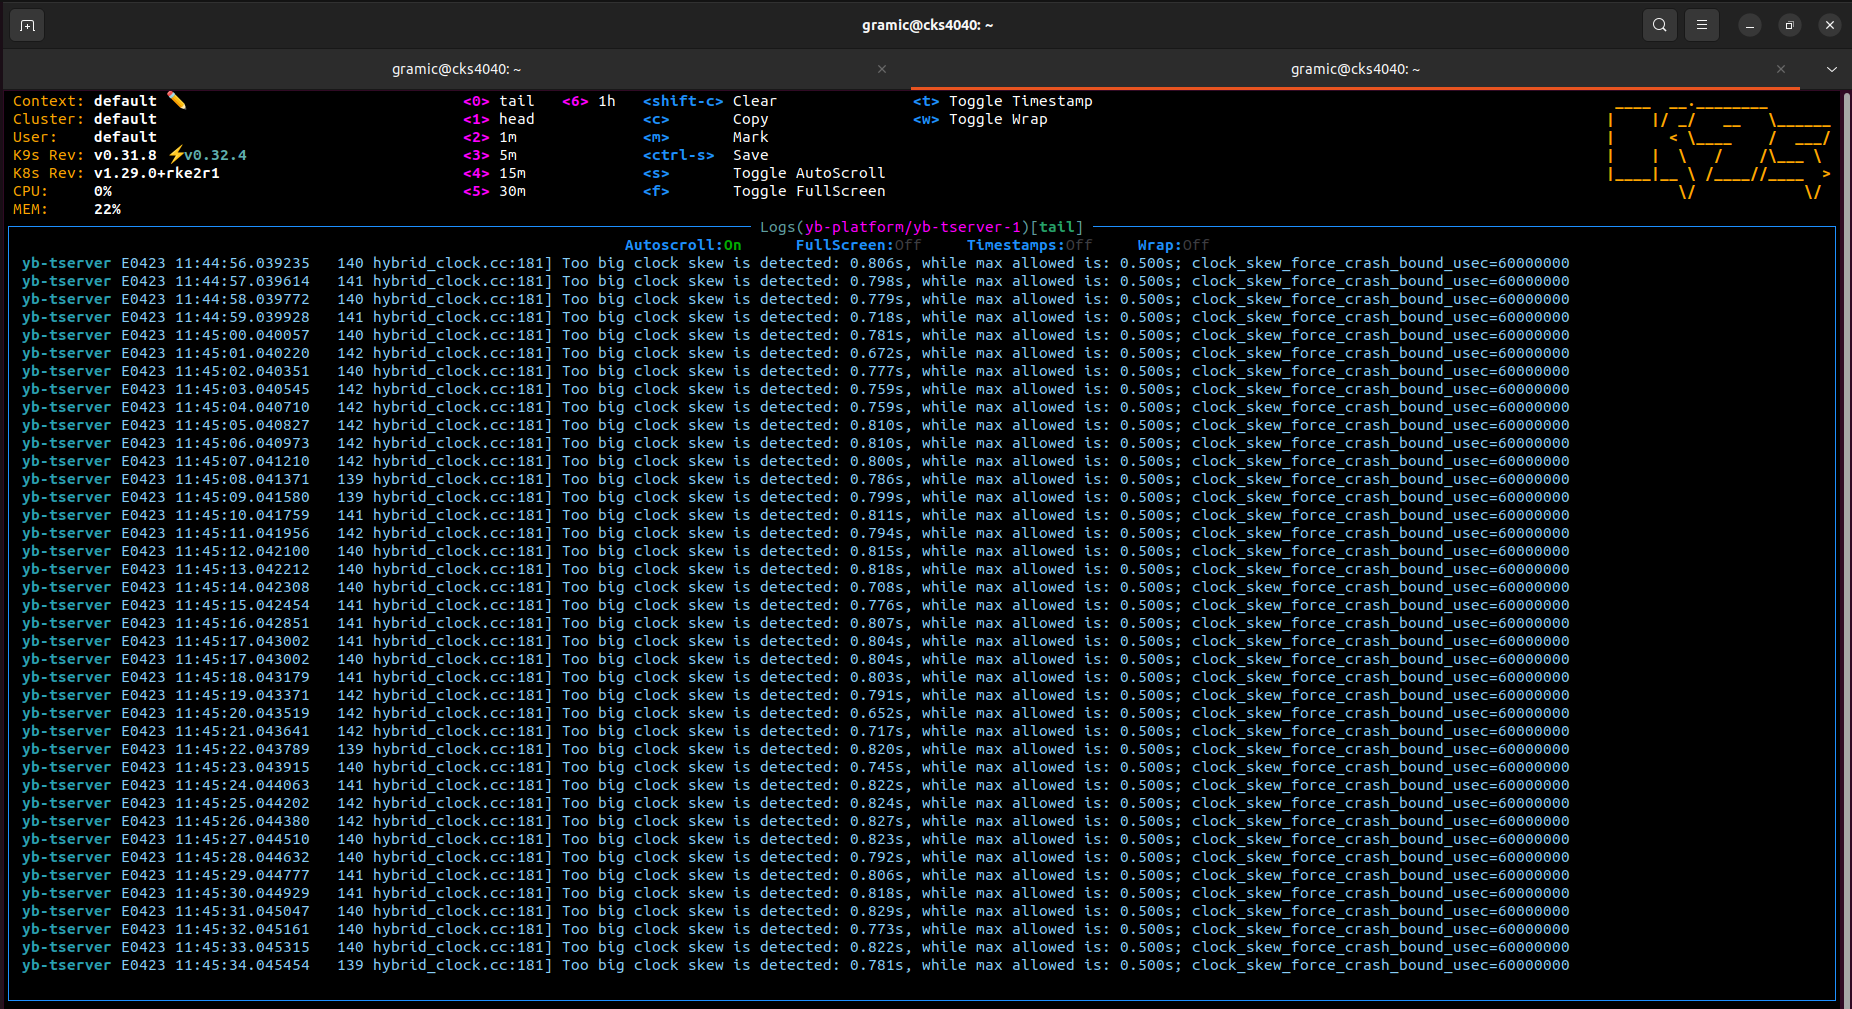
\includegraphics[width=0.47\linewidth]{source/appendix/evaluation_testing/yugabytedb_yb-tserver-1_sks1184_clock_error} }}%
%        \caption{YugabyteDB - Too big clock skew is detected - Node}
%        \label{fig:yugabytedb_sks1184_clock_error}
%    \end{figure}
    YugabyteDB erlaubt in so einem Fall keine Zugriffe mehr auf den Cluster.\\
    So wird verhindert, dass der Cluster korrumpiert wird.
\end{flushleft}
\subsection{Installation verschiedener Lösungen}
\subsection{Gegenüberstellung der Lösungen}
\subsection{Entscheid}